\documentclass[tikz,border=3pt]{standalone}
\usepackage[utf8]{inputenc}
\usepackage[T1]{fontenc}
\usepackage{lmodern}
\renewcommand{\familydefault}{\sfdefault}
\usepackage{sansmath}\sansmath
\usepackage{chemfig}
\usepackage{pgfplots}\pgfplotsset{compat=1.18,/pgf/number format/use comma,/pgf/number format/1000 sep={.}}
\usetikzlibrary{arrows.meta,calc,positioning,decorations.pathmorphing,patterns}
% paleta del sitio
\definecolor{nar}{HTML}{E8680C}\definecolor{narc}{HTML}{FFB35C}\definecolor{hielo}{HTML}{FFF3E8}
\definecolor{tinta}{HTML}{1D1D1F}\definecolor{gris}{HTML}{6E6E73}\definecolor{lila}{HTML}{7C5CF0}
\definecolor{azul}{HTML}{2F6FD6}\definecolor{menta}{HTML}{17A673}\definecolor{coral}{HTML}{E8342A}
\begin{document}
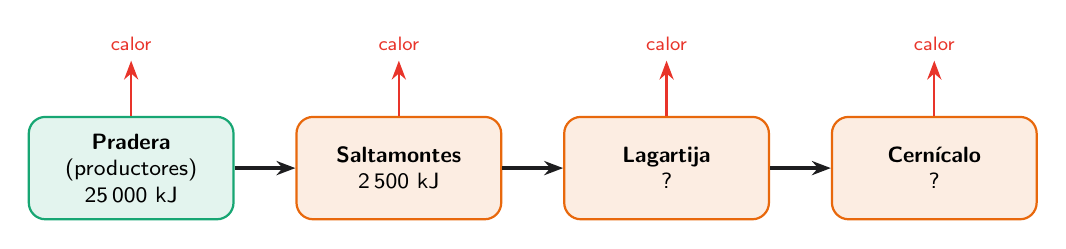
\begin{tikzpicture}[font=\small,>={Stealth[length=2.4mm]}]
\tikzset{niv/.style={draw=#1,fill=#1!12,thick,rounded corners=6pt,minimum width=2.6cm,minimum height=1.3cm,align=center,font=\footnotesize}}
\node[niv=menta] (P) at (0,0) {\textbf{Pradera}\\(productores)\\25\,000 kJ};
\node[niv=nar] (C1) at (3.4,0) {\textbf{Saltamontes}\\2\,500 kJ};
\node[niv=nar] (C2) at (6.8,0) {\textbf{Lagartija}\\?};
\node[niv=nar] (C3) at (10.2,0) {\textbf{Cernícalo}\\?};
\draw[->,very thick,tinta] (P) -- (C1); \draw[->,very thick,tinta] (C1) -- (C2); \draw[->,very thick,tinta] (C2) -- (C3);
\foreach \n in {P,C1,C2,C3} \draw[->,thick,coral] (\n.north) -- ++(0,0.7) node[anchor=south,font=\scriptsize,text=coral] {calor};
\end{tikzpicture}
\end{document}
